\documentclass[10pt,a4paper]{article}
\usepackage[left=2cm,right=2cm,top=2cm,bottom=2cm]{geometry}
\usepackage[dvipsnames]{xcolor}
\usepackage[fleqn]{mathtools}
\usepackage{booktabs}
\usepackage{amsmath}
\usepackage{latexsym}
\usepackage{graphicx}
\usepackage{nccmath}
\usepackage{multicol}
\usepackage{listings}
\usepackage{tasks}
\usepackage{color}
\usepackage{float}
\usepackage{lipsum}

\definecolor{colorIPN}{rgb}{0.5, 0.0,0.13}
\definecolor{colorESCOM}{rgb}{0.0, 0.5,1.0}
\graphicspath{ {imagenes/} }

\begin{document}
%#########################################################
\begin{titlepage}
	\centering
	{ \huge \bfseries \color{colorIPN}{Instituto Politécnico Nacional} \par}
	{ \Large \bfseries  \color{colorESCOM}{Escuela Superior de Cómputo} \par }
	\vspace{1cm}
	{\huge\Large \color{colorIPN}{Web App Development}.\par}
	\vspace{1.5cm}
	{\huge\Large  \color{colorESCOM}{PRACTICA 1: EVENTOS SERVLET}\par}
		\vspace{2cm}
	{\Large\itshape \color{colorIPN}{Profesor: M. en C. José Asunción Enríquez Zárate}\par} \hfill \break
	\vspace{2cm}
	{\Large\itshape \color{colorIPN}{Alumno: Atziri Pérez García}\par} \hfill \break
	{\Large\itshape \color{colorIPN}{atziripg.99@gmail.com}\par} \hfill \break
	{\Large\itshape \color{colorIPN}{3CM4} \par}
	\vfill
	{\large \color{colorIPN}{\today}\par} 
	\vfill
\end{titlepage}

\renewcommand\lstlistingname{Quelltext} 


\lstset{ 
	language=Java,
	basicstyle=\small\sffamily,
	numbers=left,
	numberstyle=\tiny,
	frame=tb,
	tabsize=4,
	columns=fixed,
	showstringspaces=false,
	showtabs=false,
	keepspaces,
	commentstyle=\color{Violet},
	keywordstyle=\color{colorIPN} \bfseries,
	stringstyle=\color{colorESCOM}
}

\settasks{
	counter-format=(tsk[r]),
	label-width=4ex
}
\tableofcontents 
\pagebreak
\listoffigures
\pagenumbering {arabic}

\pagebreak

%################################################
\section{\color{colorIPN}{Introducción}}
La presente práctica tiene como objetivo realizar un proyecto que donde se hagan las acciónes básicas CRUD (Create, Retrieve, Update y Delete).
Se pondrá en práctica el uso de muchas herramientas para la realización de páginas web como el servidor de aplicación Apache Tomcat, el API JDBC para crear conexión a base de datos, uso se servlets para manejar la funcionalidad de la página web, HTML para el diseño, así como frameworks para mejorar la presentación de la Web GUI como lo es Bootstrap (Front End) y validaciones en los forms.
El principal uso del proyecto es administrar los eventos realizados en la ESCOM, en este proyecto se realizan las funciones básicas:
\begin{itemize}
    \item Mostar eventos
    \item Agregar un evento nuevo
    \item Eliminar evento
    \item Actulizar evento
    \item Ver datos de un evento en específico
\end{itemize}
Cada acción tiene una interfaz diferente para un mejor y más fácil manejo del usuario.
 
\pagebreak

%################################################
\section{\color{colorIPN}{Conceptos}}
Como se mencióno, se hizo uso de varias tecnologías para realizar el proyecto, las cuales explicaremos más a fondo
\subsection{ \color{colorESCOM}{Apache Tomcat}}
El software Apache Tomcat es una implementación de código abierto de las tecnologías Java Servlet, JavaServer Pages, Java Expression Language y Java WebSocket. Las especificaciones de Java Servlet, JavaServer Pages, Java Expression Language y Java WebSocket se desarrollan bajo el Proceso de la comunidad Java.
Funciona como un contenedor de servlets desarrollado bajo el proyecto Jakarta en la Apache Software Foundation. Tomcat implementa las especificaciones de los servlets y de JavaServer Pages (JSP) de Oracle Corporation.
El software Apache Tomcat impulsa numerosas aplicaciones web de misión crítica a gran escala en una amplia gama de industrias y organizaciones. Algunos de estos usuarios y sus historias se enumeran en la página wiki de PoweredBy.

Apache Tomcat lo usamos como servidor de aplicación, en donde estará alojado nuestro proyecto.

\subsection{\color{colorESCOM}{JDBC}}
Java Database Connectivity (JDBC) es una API que permite la ejecución de operaciones sobre bases de datos desde el lenguaje de programación Java, independientemente del sistema operativo donde se ejecute o de la base de datos a la cual se accede, utilizando el dialecto SQL del modelo de base de datos que se utilice.

El API JDBC se presenta como una colección de interfaces Java y métodos de gestión de manejadores de conexión hacia cada modelo específico de base de datos. Un manejador de conexiones hacia un modelo de base de datos en particular es un conjunto de clases que implementan las interfaces Java y que utilizan los métodos de registro para declarar los tipos de localizadores a base de datos (URL) que pueden manejar. Para utilizar una base de datos particular, el usuario ejecuta su programa junto con la biblioteca de conexión apropiada al modelo de su base de datos, y accede a ella estableciendo una conexión; para ello provee el localizador a la base de datos y los parámetros de conexión específicos. A partir de allí puede realizar cualquier tipo de tarea con la base de datos a la que tenga permiso: consulta, actualización, creación, modificación y borrado de tablas, ejecución de procedimientos almacenados en la base de datos, etc.

\subsubsection{\color{colorESCOM}{Driver JDBC}}
Los drivers JDBC son adaptadores del lado del cliente (instalados en la máquina cliente, no en el servidor) que convierten la petición proveniente del programa JAVA a un protocolo que el SGBD pueda entender.
\begin{itemize}
    \item Driver JDBC Tipo 1 (también llamado Puente JDBC-ODBC) convierte el método JDBC a una llamada a una función ODBC. Utiliza los drivers ODBC para conectar con la base de datos.
    \item Driver JDBC Tipo 2 (también llamado driver API-Nativo) convierte el método JDBC a llamadas nativas de la API de la base de datos. Es más rápido que el puente JDBC-ODBC pero se necesita instalar la librería cliente de la base de datos en la máquina cliente y el driver es dependiente de la plataforma.
    \item Driver JDBC Tipo 3. Hace uso de un Middleware entre el JDBC y el SGBD.
    \item Driver JDBC Tipo 4 (también llamado Driver Java Puro directo a la base de datos). Es independiente a la plataforma.
\end{itemize}
\subsubsection{\color{colorESCOM}{Paquete}}
JDBC ofrece java.sql, en donde se encuentran las clases para manejar bases de datos:
\begin{itemize}
    \item DriverManager: Para cargar un driver
    \item Connection: Para establecer conexiones con las bases de datos
    \item Statement: Para ejecutar sentencias SQL y enviarlas a las BBDD
    \item PreparedStatement: La ruta de ejecución está predeterminada en el servidor de base de datos que le permite ser ejecutado varias veces
    \item ResultSet: Para almacenar el resultado de la consulta
\end{itemize}

\subsection{\color{colorESCOM}{Servlets}}
Un servlet es una clase en el lenguaje de programación Java, utilizada para ampliar las capacidades de un servidor. Aunque los servlets pueden responder a cualquier tipo de solicitudes, estos son utilizados comúnmente para extender las aplicaciones alojadas por servidores web, de tal manera que pueden ser vistos como applets de Java que se ejecutan en servidores en vez de navegadores web. Este tipo de servlets son la contraparte Java de otras tecnologías de contenido dinámico Web, como PHP y ASP.NET.
\subsubsection{\color{colorESCOM}{Ciclo de vida}}
\begin{enumerate}
    \item Inicializar el servlet: 
Cuando un servidor carga un servlet, ejecuta el método init del servlet. El proceso de inicialización debe completarse antes de poder manejar peticiones de los clientes, y antes de que el servlet sea destruido.

    \item Interactuar con los clientes: 
Después de la inicialización, el servlet puede dar servicio a las peticiones de los clientes. Estas peticiones serán atendidas por la misma instancia del servlet, por lo que hay que tener cuidado al acceder a variables compartidas, ya que podrían darse problemas de sincronización entre requerimientos simultáneos.

    \item Destruir el servlet: 
Los servlets se ejecutan hasta que el servidor los destruye, por cierre del servidor o bien a petición del administrador del sistema. Cuando un servidor destruye un servlet, ejecuta el método destroy del propio servlet. Este método sólo se ejecuta una vez y puede ser llamado cuando aún queden respuestas en proceso, por lo que hay que tener la atención de esperarlas. El servidor no ejecutará de nuevo el servlet hasta haberlo cargado e inicializado de nuevo.
\end{enumerate}

\subsection{\color{colorESCOM}{Bootstrap}}
Bootstrap es una biblioteca multiplataforma o conjunto de herramientas de código abierto para diseño de sitios y aplicaciones web. Contiene plantillas de diseño con tipografía, formularios, botones, cuadros, menús de navegación y otros elementos de diseño basado en HTML y CSS, así como extensiones de JavaScript adicionales. A diferencia de muchos frameworks web, solo se ocupa del desarrollo front-end.
\pagebreak

%################################################
\section{\color{colorIPN}{Desarrollo}}
A continuacipon se explica el proceso que se siguió para realizar este proyecto paso a paso:
	\item  Uso del Apache Tomcat: Como sabemos, usamos el IDE Apache NetBeans para desarrollar el proyecto, por lo que es necesario conectar Apache Tomat al IDE que estemos ocupando. En la Tarea 1 se explicó la instalación y la conexión con el IDE. En la figura podemos ver que el servidor esta funcionando con normalidad.
	\begin{figure}[H]
    	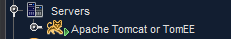
\includegraphics[scale=.8]{images/servidor.png}
    	\centering \linebreak \linebreak 
    	\caption{Tomcat funcionando}
    	\label{img:tomcat}
    \end{figure}  \hfill

	\subection{\color{colorIPN}{Evento}}
	Después de crear empaquetados para tener más organizado el proyecto, continuamos haciendo la primera clase de nuestro proyecto, la cual es Evento. En esta clase encontramos las funciones basicas de una clase como el constructor , los getter y los setter. Aquí mismo podemos visualizar cuales son los datos que manipularemos de un evento, los cuales son:
	\begin{itemize}
	    \item idEvento
        \item nombreEvento
        \item sede
        \item duracion
        \item fechaInicio
        \item fechaTermino
	\end{itemize}
    	\begin{lstlisting}
            
            /**
             *
             * @author Atziri Perez
             */
            public class Evento implements Serializable{
                private int idEvento;
                private String nombreEvento;
                private String sede;
                private double duracion;
                private Date fechaInicio;
                private Date fechaTermino;
                
                public Evento(){}
            
                public int getIdEvento() {
                    return idEvento;
                }
            
                public void setIdEvento(int idEvento) {
                    this.idEvento = idEvento;
                }
            
                public String getNombreEvento() {
                    return nombreEvento;
                }
            
                public void setNombreEvento(String nombreEvento) {
                    this.nombreEvento = nombreEvento;
                }
            
                public String getSede() {
                    return sede;
                }
            
                public void setSede(String sede) {
                    this.sede = sede;
                }
            
                public double getDuracion() {
                    return duracion;
                }
            
                public void setDuracion(double duracion) {
                    this.duracion = duracion;
                }
            
                public Date getFechaInicio() {
                    return fechaInicio;
                }
            
                public void setFechaInicio(Date fechaInicio) {
                    this.fechaInicio = fechaInicio;
                }
            
                public Date getFechaTermino() {
                    return fechaTermino;
                }
            
                public void setFechaTermino(Date fechaTermino) {
                    this.fechaTermino = fechaTermino;
                }
            
               
                @Override
                public String toString() {
                    StringBuilder sb = new StringBuilder();
                    sb.append("Evento{idEvento=").append(idEvento).append("\n");
                    sb.append(", nombreEvento=").append(nombreEvento).append("\n");
                    sb.append(", sede=").append(sede).append("\n");
                    sb.append(", duracion=").append(duracion).append("\n");
                    sb.append(", fechaInicio=").append(fechaInicio).append("\n");
                    sb.append(", fechaTermino=").append(fechaTermino).append("\n");
                    sb.append('}');
                    return sb.toString();
                }
              
            }
    	\end{lstlisting}
	\subection{\color{colorIPN}{EventoDAO}} 
	Después de crear la clase Evento, debemos hacer los métodos para lograr el CRUD que necesitamos, así como la conexión a la base de datos. Estos métodos de conexión y los métodos de CRUD se incluyeron en otra clase llamada EventoDAO. Cabe mencionar que se realizó la separación solo para abstraer la clase Evento, y mantener separados los métodos y la conexión de BD.
    \begin{lstlisting}
                /*
 * To change this license header, choose License Headers in Project Properties.
 * To change this template file, choose Tools | Templates
 * and open the template in the editor.
 */
package com.ipn.mx.modelo.dao;

import com.ipn.mx.modelo.dto.Evento;
import java.sql.Connection;
import java.sql.DriverManager;
import java.sql.PreparedStatement;
import java.sql.ResultSet;
import java.sql.Date;
import java.sql.SQLException;
import java.util.List;
import java.util.ArrayList;
import java.util.logging.Level;
import java.util.logging.Logger;
/**
 *
 * @author Atziri Perez
 */
public class EventoDAO {
    public static final String SQL_INSERT ="insert into evento(nombreEvento, sede, duracion,fechaInicio,fechaTermino)" + " values(?, ?, ?, ?, ?)"; 
    public static final String SQL_UPDATE ="update evento set nombreEvento = ?, sede = ?, duracion = ?, fechaInicio = ?, fechaTermino = ? where idEvento = ?"; 
    public static final String SQL_DELETE ="delete from evento where idEvento = ?";  
    public static final String SQL_SELECT_ALL ="select * from evento"; 
    public static final String SQL_SELECT ="select * from evento where idEvento = ?"; 

    private Connection conexion = null;
    private void obtenerConexion(){
        String usr = "root";
        String pwd = "password";
        String driver = "com.mysql.cj.jdbc.Driver";
        String url ="jdbc:mysql://localhost:3306/ProyectoBase3CM4?serverTimezone=America/Mexico_City&useUnicode=true&useJDBCCompliantTimezoneShift=true&useLegacyDatetimeCode=false&useSSL=false";       
        try {
            Class.forName(driver);
            conexion = DriverManager.getConnection(url, usr, pwd);
        } catch (ClassNotFoundException | SQLException ex) {
            Logger.getLogger(Evento.class.getName()).log(Level.SEVERE, null, ex);
        }
    }
    
    public void create(Evento e)throws SQLException{
        obtenerConexion();
        PreparedStatement ps = null;
        try {
            ps = conexion.prepareStatement(SQL_INSERT);
            ps.setString(1, e.getNombreEvento());
            ps.setString(2, e.getSede());
            ps.setDouble(3, e.getDuracion());
            ps.setDate(4, e.getFechaInicio());
            ps.setDate(5, e.getFechaTermino());
            ps.executeUpdate();
        } finally{
            if (ps!=null)
                ps.close();
            if(conexion!=null)
                conexion.close();
        }
    }
    public void update(Evento e) throws SQLException{
        obtenerConexion();
        PreparedStatement ps = null;
        try {
            ps = conexion.prepareStatement(SQL_UPDATE);
            ps.setString(1, e.getNombreEvento());
            ps.setString(2, e.getSede());
            ps.setDouble(3, e.getDuracion());
            ps.setDate(4, e.getFechaInicio());
            ps.setDate(5, e.getFechaTermino());
            ps.setInt(6, e.getIdEvento());
            ps.executeUpdate();
        } finally{
            if (ps!=null)
                ps.close();
            if(conexion!=null)
                conexion.close();
        }
    }
     
    public void delete(Evento e) throws SQLException{
        obtenerConexion();
        PreparedStatement ps = null;
        try {
            ps = conexion.prepareStatement(SQL_DELETE);
            ps.setInt(1, e.getIdEvento());
            ps.executeUpdate();
        } finally{
            if (ps!=null)
                ps.close();
            if(conexion!=null)
                conexion.close();
        }
    }
     
    public List readAll()throws SQLException{
        obtenerConexion();
        PreparedStatement ps = null;
        ResultSet rs = null;
        try{
            ps = conexion.prepareStatement(SQL_SELECT_ALL);
            rs = ps.executeQuery();
            List resultados = obtenerResultados(rs);
            if(resultados.size() > 0)
                return resultados;
            else
                return null;
        }finally{
            if(rs!=null)
                rs.close();
            if(ps!=null)
                ps.close();
            if(conexion!= null)
                conexion.close();
        }
    }
            
    public Evento read(Evento e) throws SQLException{
        obtenerConexion();
        PreparedStatement ps = null;
        ResultSet rs = null;
        try{
            ps = conexion.prepareStatement(SQL_SELECT);
            ps.setInt(1, e.getIdEvento());
            rs = ps.executeQuery();
            List resultados = obtenerResultados(rs);
            if(resultados.size()>0)
                return (Evento)resultados.get(0);
            else
                return null;
        }finally{
            if(rs!=null)
                rs.close();
            if(ps!=null)
                ps.close();
            if(conexion!= null)
                conexion.close();
        }
    }
       
    private List obtenerResultados(ResultSet rs) throws SQLException{
        List resultados = new ArrayList();
        while(rs.next()){
            Evento e = new Evento();
            e.setIdEvento(rs.getInt("idEvento"));
            e.setNombreEvento(rs.getString("nombreEvento"));
            e.setSede(rs.getString("sede"));
            e.setDuracion(rs.getDouble("duracion"));
            e.setFechaInicio(rs.getDate("fechaInicio"));
            e.setFechaTermino(rs.getDate("fechaTermino"));
            resultados.add(e);
        }
        return resultados;
    }
    
    public static void main(String[] args) {
        Evento e = new Evento();
        e.setIdEvento(1);
        e.setNombreEvento("Hackaton");
        e.setSede("Auditorio ESCOM");
        e.setDuracion(5);
        e.setFechaInicio(Date.valueOf("2020-10-16"));
        e.setFechaTermino(Date.valueOf("2020-10-24"));  
        
        EventoDAO dao = new EventoDAO();
        try {
            dao.create(e);
        } catch (SQLException ex) {
            Logger.getLogger(Evento.class.getName()).log(Level.SEVERE, null, ex);
        }
    }
}
    \end{lstlisting}
    Como se puede ver, en EventoDAO.java es en donde se hace uso del API JDBC y se hace la conexión con la base de datos que ya existe en el usuario que se determinó en el código.
    
    Podemos ver también los metodos create(), delete(),update(), read(), readAll() en donde conectamos con la base de datos y ejecutamos la consulta correspondiente.
    Es importante darse cuenta que aun no trabajamos con ningun aspecto WEB, solo se está desarrollando la parte funcional de nuestro proyecto, por consiguiente es recomendable probar la funcionalidad del proyecto hasta este punto paraa verificar que las acciones CRUD se hacen corretamente en la base de datos.
    
   \subection{\color{colorIPN}{Servlet}} Una vez que estamos seguros que el proyecto funciona bien, podemos empezar a trabajar con servlets para ir formando la estructura de nuestra página web.
    Creamos un servlet en donde determinamos las acciones principales de este:
    \begin{lstlisting}
        String accion = request.getParameter("accion");
        if (accion.equals("listaDeEventos")) {
            listaDeEventos(request, response);
        } else {
            if (accion.equals("nuevo")) {
                agregarEvento(request, response);
            } else {
                if (accion.equals("eliminar")) {
                    eliminarEvento(request, response);
                } else {
                    if (accion.equals("actualizar")) {
                        actualizarEvento(request, response);
                    }
                    if (accion.equals("guardar")) {
                        almacenarEvento(request, response);
                    }
                    if (accion.equals("ver")) {
                        mostrarEvento(request, response);
                    }
                }
            }
        }
    \end{lstlisting}
    Cada uno de los métodos mostrados en el código anterior, están determinados en este mismo servlet, en cada uno incluimos código html para formar la estructura de la página web respecto al Front-End.
    \subsubsection{\color{colorIPN}{listaDeEventos}}
    listaDeEventos será el home de nuestra página, es donde se mostrará el listado de los eventos que se encuentran en la base de datos, así como la opción de realizar acciones a cada uno (Ver, Eliminar o Editar). Esta es nuestra vista principal.
    \begin{lstlisting}
    private void listaDeEventos(HttpServletRequest request, HttpServletResponse response) throws IOException {
        ...
        int idEvento;
            String nombreEvento;
            String sede;
            double duracion;
            Date fechaInicio;
            Date fechaTermino;
        
            EventoDAO dao = new EventoDAO();
            List lista = dao.readAll();
        for (int i = 0; i < lista.size(); i++) {
            Evento evento = (Evento) lista.get(i);
            idEvento = evento.getIdEvento();
            nombreEvento = evento.getNombreEvento();
            sede = evento.getSede();
            duracion = evento.getDuracion();
            fechaInicio = evento.getFechaInicio();
            fechaTermino = evento.getFechaTermino();
    ..}
    \end{lstlisting}
    Dejando de lado el código html, podemos ver que se hace uso del método readAll, el cual es una consulta SELECT a la base de datos, la cual la desarrollamos en EventDAO.java
    \subsubsection{\color{colorIPN}{agregarEvento}}
    El método agregarEvento, solo nos redirige a otro form html para crear un nuevo evento:
    \begin{lstlisting}
    private void agregarEvento(HttpServletRequest request, HttpServletResponse response) {
        try {
            request.getRequestDispatcher("eventoForm.html").forward(request, response);
        } catch (ServletException | IOException ex) {
            Logger.getLogger(Servlet.class.getName()).log(Level.SEVERE, null, ex);
        }
    \end{lstlisting}
    \subsubsection{\color{colorIPN}{eliminarEvento}}
    El método eliminatEvento, eliminará un evento tomando como parámetro el id del evento a eliminar:
    \begin{lstlisting}
        EventoDAO dao = new EventoDAO();
        Evento e = new Evento();
        try {
            e.setIdEvento(Integer.parseInt(request.getParameter("id")));
            e = dao.read(e);
            dao.delete(e);
            listaDeEventos(request, response);
        } catch (SQLException | IOException ex) {
            Logger.getLogger(Servlet.class.getName()).log(Level.SEVERE, null, ex);
        }
    \end{lstlisting}
    \subsubsection{\color{colorIPN}{almacenarEvento}}
    El método almacenarEvento hace uso de los metodos creat() y update() para almacenar un evento nuevo en la base de datos, o bien si ya existe, actualizar sus datos a los nuevo que el usuario escribió.
    Esta validación se realizó verificando si se envió como parámetro en la URL la id del evento (En caso de actualizar datos )usando el método POST:
    \begin{lstlisting}
    private void almacenarEvento(HttpServletRequest request, HttpServletResponse response) {
        EventoDAO dao = new EventoDAO();
        Evento e = new Evento();
        if (request.getParameter("id") == null || request.getParameter("id").isEmpty()) {
            e.setNombreEvento(request.getParameter("nombreEvento"));
            e.setSede(request.getParameter("sedeEvento"));
            e.setDuracion(Double.parseDouble(request.getParameter("duracion")));
            e.setFechaInicio(Date.valueOf(request.getParameter("fechaInicio")));
            e.setFechaTermino(Date.valueOf(request.getParameter("fechaTermino")));
            try {
                dao.create(e);
                response.sendRedirect("Servlet?accion=listaDeEventos");
            } catch (SQLException | IOException ex) {
                Logger.getLogger(Servlet.class.getName()).log(Level.SEVERE, null, ex);
            }
        } else {
            e.setIdEvento(Integer.parseInt(request.getParameter("id")));
            e.setNombreEvento(request.getParameter("nombreEvento"));
            e.setSede(request.getParameter("sedeEvento"));
            e.setDuracion(Double.parseDouble(request.getParameter("duracion")));
            e.setFechaInicio(Date.valueOf(request.getParameter("fechaInicio")));
            e.setFechaTermino(Date.valueOf(request.getParameter("fechaTermino")));
            try {
                dao.update(e);
                response.sendRedirect("Servlet?accion=listaDeEventos");
            } catch (SQLException | IOException ex) {
                Logger.getLogger(Servlet.class.getName()).log(Level.SEVERE, null, ex);
            }
        }
    }
    \end{lstlisting}
    \subsubsection{\color{colorIPN}{actualizat y mostrar Evento}}
    Los metoddos actualizarEvento y mostrarEvento hacen uso de update() y read() respectivamente, instanciando el objeto Evento de la misma manera que se realizó en los métodos anteriores. 
    *Para ver código, ir al código fuente
    \begin{lstlisting}
    \end{lstlisting}

%################################################
\hfill \break



\pagebreak


%################################################
\section{\color{colorIPN}{Resultados}}
Finalmente, mostramos el proyecto funcionando:
%################################################
\begin{itemize}
    \item Primero mostramos la página incial Lista de eventos donde vemos los eventos que se encuentran actualmente en la base de datos:
        \begin{figure}[H]
    	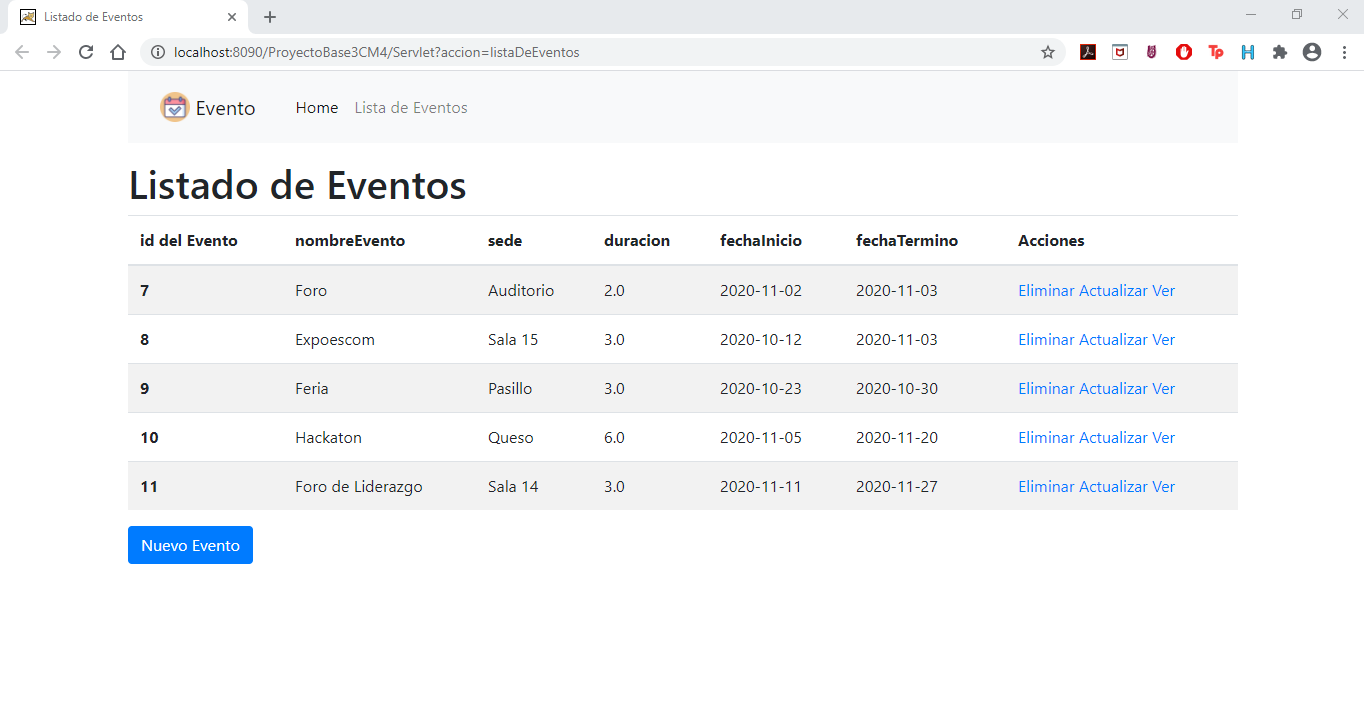
\includegraphics[scale=0.5]{images/listaDeEventos.png}
    	\centering \linebreak \linebreak 
    	\caption{Lista De Eventos}
    	\label{img:List}
    \end{figure}  \hfill
    \item Ahora agregamos un evento
        \begin{figure}[H]
    	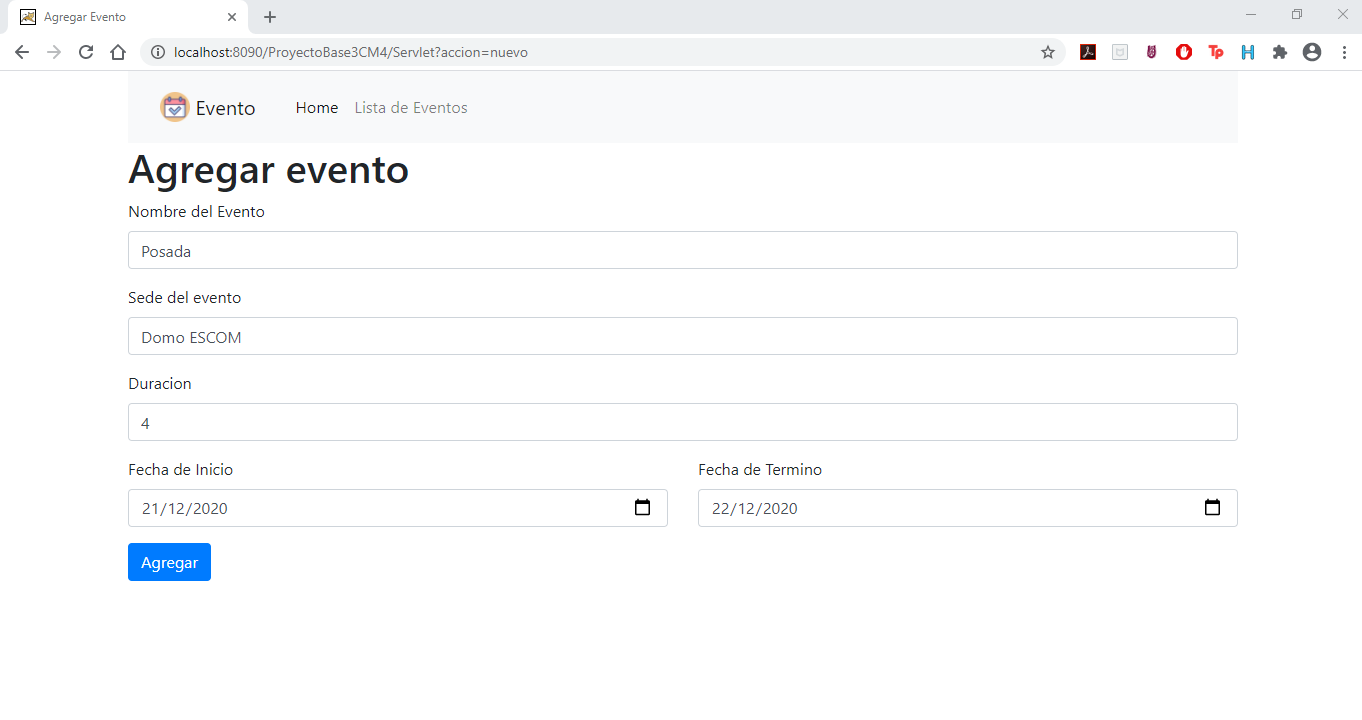
\includegraphics[scale=0.5]{images/agregarEvento.png}
    	\centering \linebreak \linebreak 
    	\caption{Agregar Evento}
    	\label{img:Add}
    \end{figure}  \hfill
    \item Ahora probemos la funcion de actualizar evento, actualizaremos el evento 7
        \begin{figure}[H]
    	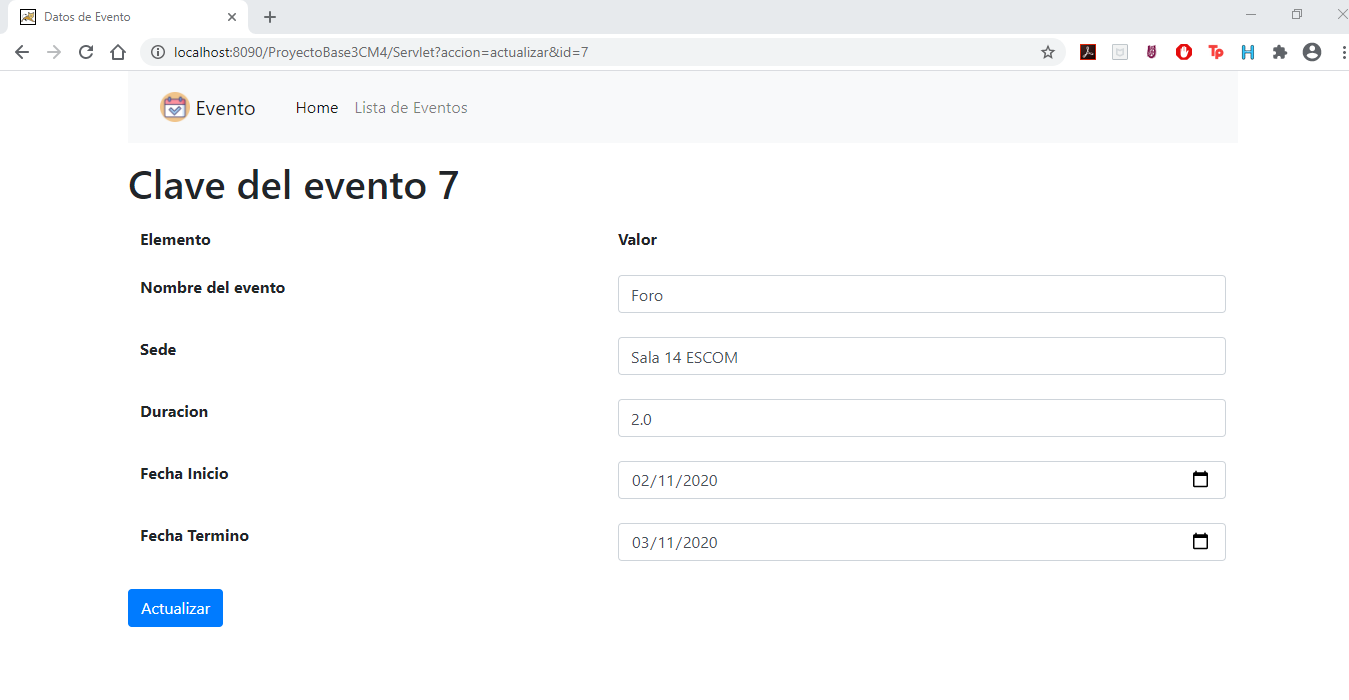
\includegraphics[scale=0.5]{images/actualizarEvento.png}
    	\centering \linebreak \linebreak 
    	\caption{Actualizar evento}
    	\label{img:update}
    \end{figure}  \hfill
    \item Continuamos mostrando la información completa de un evento, en este caso el numero 10
        \begin{figure}[H]
    	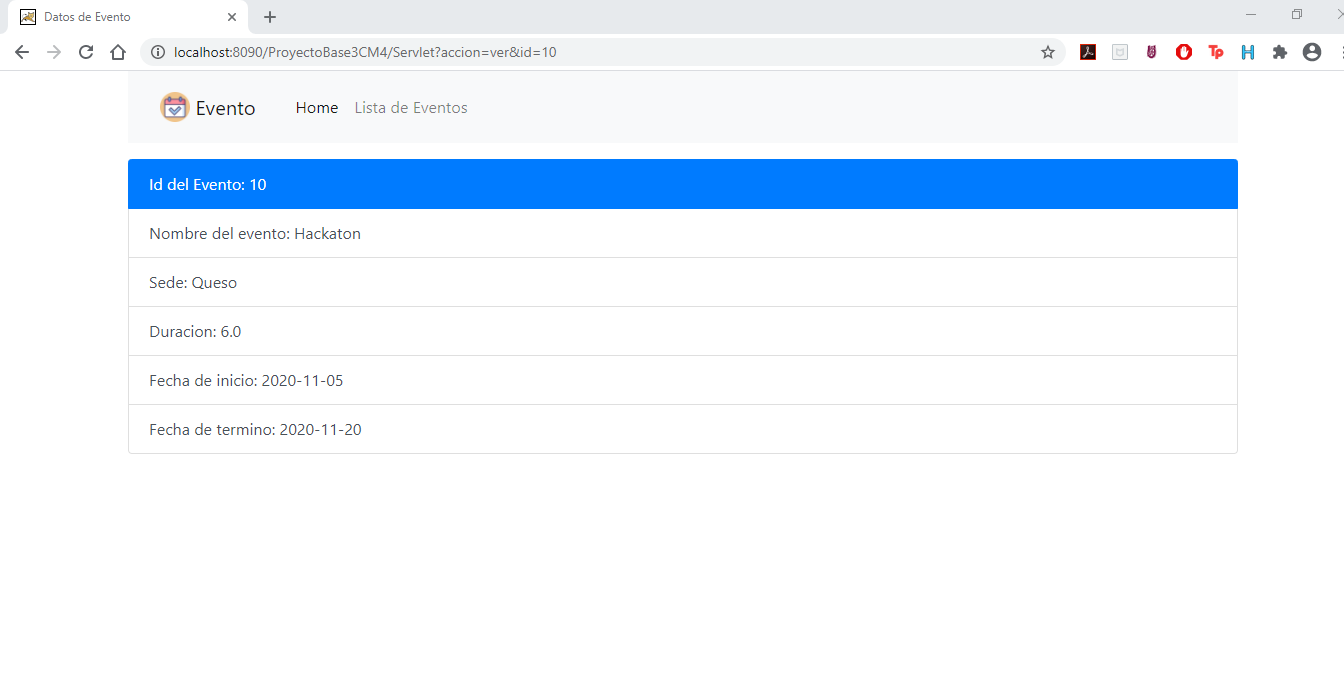
\includegraphics[scale=0.5]{images/verEvento.png}
    	\centering \linebreak \linebreak 
    	\caption{Ver evento}
    	\label{img:read}
    \end{figure}  \hfill
    \item Eliminaremos ese mismo evento, y lista de Eventos queda de la siguiente manera:
        \begin{figure}[H]
    	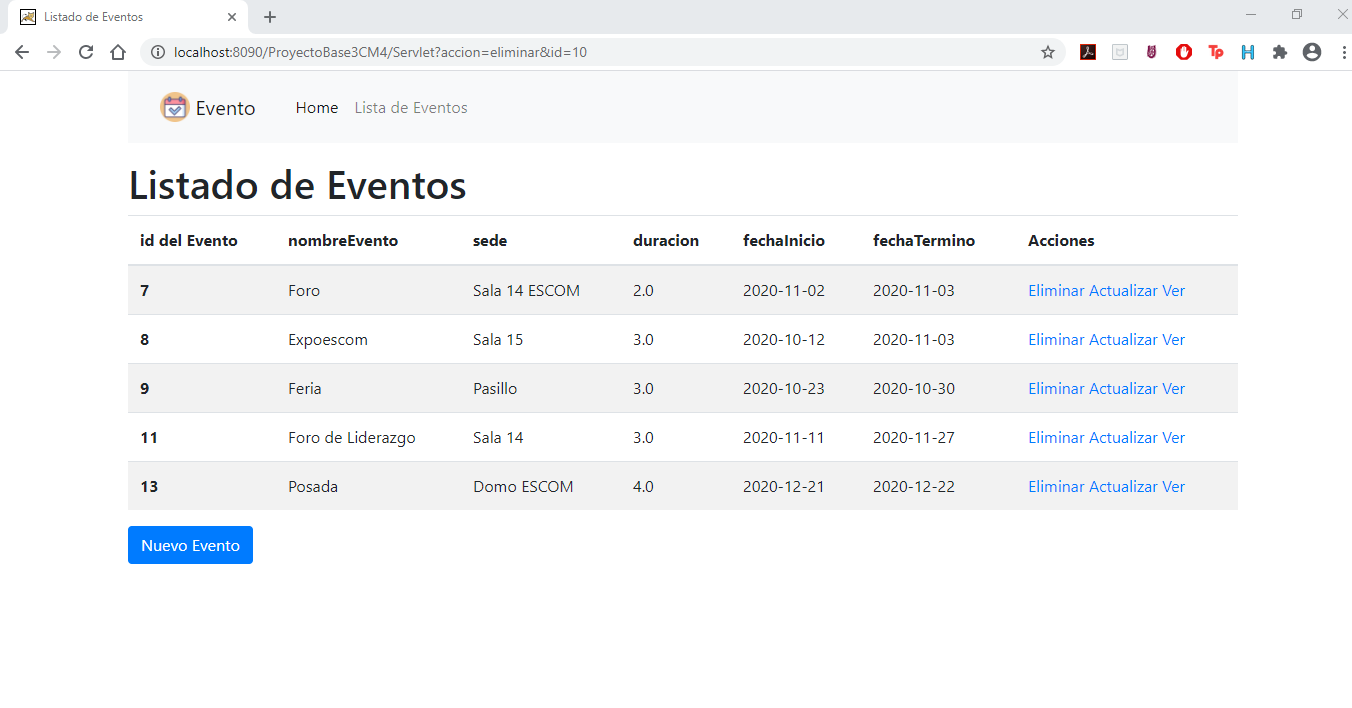
\includegraphics[scale=0.5]{images/listaDeEventos2.png}
    	\centering \linebreak \linebreak 
    	\caption{Lista de Eventos con modificaciones}
    	\label{img:final}
    \end{figure}  \hfill
\end{itemize}
\pagebreak



%################################################
\section{\color{colorIPN}{Conclusión}}
El proyceto resultó ser muy completo e integral para entender todas las tecnologías que se necesitan durante la implementación de un proyecto web.
En mi experiencia, solo estaba familiarizada con el usp de Bootstrap para la parte del front-end, sin embargo no fue dificil adaptarme a JDBC, ni a los servlets ya qe siguen la línea de las herramientas web que he utilizado (Flask para python, ASP C#, etc.)

\color{colorIPN}{
	\begin{flushright}
		\textit{
			Atziri Pérez García
		}
	\end{flushright} \hfill \break
}

\pagebreak

%################################################

\section{\color{colorIPN}{Referencias Bibliográficas}}
\color{colorESCOM}{
	\begin{thebibliography}{10}
		\bibitem[Tomcat, 2019]{Tomcat}
	    Apache Tomcat
		\newblock {\em Tomcat 9}
		\newblock Apache Tomcat Disponible en:
		\newblock {\em https://tomcat.apache.org/}
		\bibitem[Bootstrap, 2020]{Bootstrap}
		\newblock {\em Bootstrap}
		\newblock Disponible en:
		\newblock {\em https://getbootstrap.com}
		\bibitem[JDBC, 2020]{Bootstrap}
		\newblock {\em ¿Que es JDBC?}
		\newblock Disponible en:
		\newblock {\em http://profesores.fi-b.unam.mx/sun/Downloads/Java/jdbc.pdf}

	
	\end{thebibliography}
}

\end{document}
